\documentclass[usenatbib]{mn2e} 
\usepackage{amsmath} 
\usepackage{amssymb} 
\usepackage{graphics}
\usepackage{graphicx}
\usepackage{epsfig} 
\usepackage{float} 
\def\be{\begin{equation}}
\def\ee{\end{equation}}
\def\ba{\begin{eqnarray}}
\def\ea{\end{eqnarray}}
\bibliographystyle{mn2e}
% To highlight comments 
\usepackage{color}
\definecolor{red}{rgb}{1,0.0,0.0}
\newcommand{\red}{\color{red}}
\definecolor{blue}{rgb}{0.1,0.3,0.9}
\newcommand{\blue}{\color{blue}}

\usepackage[normalem]{ulem}
\definecolor{darkgreen}{rgb}{0.0,0.5,0.0}
\newcommand{\SRK}[1]{\textcolor{darkgreen}{\bf SRK: \textit{#1}}}
\newcommand{\SRKED}[1]{\textcolor{darkgreen}{\bf #1}}
\newcommand{\LCDM}{$\Lambda$CDM~}
\newcommand{\beq}{\begin{eqnarray}}  
\newcommand{\eeq}{\end{eqnarray}}  
\newcommand{\zz}{$z\sim 3$} 
\newcommand{\apj}{ApJ}  
\newcommand{\apjs}{ApJS}  
\newcommand{\apjl}{ApJL}  
\newcommand{\aj}{AJ}  
\newcommand{\mnras}{MNRAS}  
\newcommand{\mnrassub}{MNRAS accepted}  
\newcommand{\aap}{A\&A}  
\newcommand{\aaps}{A\&AS}  
\newcommand{\araa}{ARA\&A}  
\newcommand{\nat}{Nature}  
\newcommand{\physrep}{PhR}
\newcommand{\pasp}{PASP}    
\newcommand{\pasj}{PASJ}    
\newcommand{\avg}[1]{\langle{#1}\rangle}  
\newcommand{\nscatt}{\langle N_{\rm  scatt}\rangle}
\newcommand{\ly}{{\ifmmode{{\rm Ly}\alpha~}\else{Ly$\alpha$~}\fi}}
\newcommand{\hMpc}{{\ifmmode{h^{-1}{\rm Mpc}}\else{$h^{-1}$Mpc }\fi}}   
\newcommand{\hGpc}{{\ifmmode{h^{-1}{\rm Gpc}}\else{$h^{-1}$Gpc }\fi}}   
\newcommand{\hmpc}{{\ifmmode{h^{-1}{\rm Mpc}}\else{$h^{-1}$Mpc }\fi}}  
\newcommand{\hkpc}{{\ifmmode{h^{-1}{\rm kpc}}\else{$h^{-1}$kpc }\fi}}  
\newcommand{\hMsun}{{\ifmmode{h^{-1}{\rm
        {M_{\odot}}}}\else{$h^{-1}{\rm{M_{\odot}}}$}\fi}}   
\newcommand{\hmsun}{{\ifmmode{h^{-1}{\rm
        {M_{\odot}}}}\else{$h^{-1}{\rm{M_{\odot}}}$}\fi}}   
\newcommand{\Msun}{{\ifmmode{{\rm {M_{\odot}}}}\else{${\rm{M_{\odot}}}$}\fi}}  
\newcommand{\msun}{{\ifmmode{{\rm {M_{\odot}}}}\else{${\rm{M_{\odot}}}$}\fi}}  
\newcommand{\lya}{{Lyman$\alpha$~}}
\newcommand{\clara}{{\texttt{CLARA}}~}
\newcommand{\rand}{{\ifmmode{{\mathcal{R}}}\else{${\mathcal{R}}$ }\fi}}  
\newcommand{\hs}{{\hspace{1mm}}}  
\newcommand{\kms}{{\ifmmode{{\mathrm{\,km\ s}^{-1}}}\else{\,km~s$^{-1}$}\fi}}

% definition to produce a "less than or similar to" symbol
\def\lsim{~\rlap{$<$}{\lower 1.0ex\hbox{$\sim$}}}

% definition to produce a "greater than or similar to" symbol
\def\gsim{~\rlap{$>$}{\lower 1.0ex\hbox{$\sim$}}}

\begin{document}

\title[Rotation in the Lyman-$\alpha$ line]{The impact of gas bulk
  rotation on the Lyman-$\alpha$ line} 
\author[Garavito-Camargo, Forero-Romero \& Dijkstra]{
\parbox[t]{\textwidth}{\raggedright 
  Nicolas Garavito-Camargo$^{1}$,
  Jaime E. Forero-Romero$^{1}$ and 
  Mark Dijkstra$^2$
}
\vspace*{6pt}\\
$^{1}$Departamento de F\'{i}sica, Universidad de los Andes, Cra. 1
No. 18A-10, Edificio Ip, Bogot\'a, Colombia \\
$^2$
}
\maketitle

\begin{abstract}
Rotation is present in the gas kinematics of galaxies up to the
highest redshifts. In this paper we present for the first time 
radiative transfer calculations that show the impact of gas bulk rotation on
the morphology of the Lyman $\alpha$ line. To this end we model a
galaxy as an homogeneous sphere composed as an homogeneous mixture of
dust and hydrogen at a constant temperature. These spheres have a
solid-body rotation with linear velocities at the surface in the range
$0-300$ \kms and neutral hydrogen optical depths in the range
$\tau_{\rm H}=10^{5}-10^{7}$. We consider radiation sources both in
the center of the rotating cloud and also homogeneously distributed in
the volume. We find that higher rotational velocities increase the
width of each peak in the outgoing line profile while it also
increases the amount of Lyman alpha photons escaping in the line
center. This trends makes that for high rotational velocities and
large Hydrogen optical depths the double peak of the line tends to be
erased an be replaced by a single peak a the line center. This trend
is more pronounced for radiation sources homogeneously
distributed. Concerning the escape fraction we find that rotation does
not have any effect, provided that all the sources are centrally
emitted. However, in the case of homogeneously emittedsources we
measure an increase of about a factor of $2$ in the escape  fraction
for higher rotational velocity values. This work shows that gas bulk
rotation has a non negligible impact on the shape of the Lyman
$\alpha$ line.   
\end{abstract}
\begin{keywords}
galaxies: high-redshift - galaxies: star formation - line: formation
\end{keywords}


\section{Introduction}
\label{sec:intro}

The detection of strong \ly emission lines has become an essential
method in extragalactic astronomy to find distant star-forming
galaxies
\citep{PartridgePeebles,Rhoads00,Gawiser2007,Koehler2007,Ouchi08,Yamada2012,Schenker2012}.
The galaxies detected using this method receive the 
name of \ly emitters (LAEs). A detailed examination of this galaxy
population has diverse implications for galaxy formation, reonization
and the large scale structure of the Universe. Attempts to fully
exploit the physical information included in the \ly line require an
understading of all the physical factors involved in shaping the
line. Due to the resonant nature of this line, these physical factors
include temperature, density and bulk velocity field of the neutral
Hydrogen in the emitting galaxy and its surroundings.


A basic understanding for the quantitative behaviour of the \ly line
has been reached through analytical studies in the case of a static
configurations, such as uniform slabs
\citep{Harrington73,Neufeld90} and  uniform spheres
\citep{Dijkstra06}. Analytical studies of configurations including
some kind of bulk flow only include the case of a sphere with a Hubble
like expansion flow \citep{LoebRybicki}. 

A more detailed quantification of the \ly line has been reached using
Monte Carlo simulations \citep{Auer68,Avery68,Adams72}. In the last
two decades these studies have become more popular due to the
availability of computing power. Early into the 21st century the first
studies focused on on homogeneous and static media
\citep{Ahn00,Ahn01,Zheng02}. Later on the effects of clumpy media
\citep{Hansen06} and expanding/contracting shell/spherical geometries started to
be studied \citep{Verhamme06,Dijkstra06}. Similar codes have applied
these results to semi-analytical models of galaxy formation \citep{Orsi12} and
results of large hydrodynamical simulations
\citep{CLARA,Forero12,Behrens13}. Recently Monte Carlo codes have also
been applied to the results of high resolution hydrodynamical
simulations \citep{Laursen09,Barnes11,Verhamme12,Yajima12}. Recent developments have been
focused on the study of clumpy outflows \citep{DijkstraKramer}and
anisotropic velocity configurations \citep{Zheng2013}.

The recent studies of galaxies in hydrodynamical simulations
\citep{Laursen09,Barnes11,Verhamme12,Yajima12} have all shown
systematic variations in the \ly line with the viewing angle. These
variations are a complex superpositions of anisotropic density
configurations (i.e. edge-on vs. face-on view of a galaxy), the
inflows observaed by gas cooling and the outflows included in the
supernova feedback process of the simulation. These bulk flows
physically correspond to the circumgalactic and intergalactic medium
(CGM and IGM). These effects have been systematically studied
different anisotropic models of hydrogen clouds  varying the density
and wind characteristics \citep{Zheng2013}.

However, in all these systematics efforts the effect of rotation,
which is an ubiquitous feature in galaxies, has not been
systematically studied. The processing of the \ly photons in a
rotating interstellar medium (ISM) must have an impact in the line
morphology. It is necessary to investigate to what extent bulk gas
rotation has an measurable impact in the \ly alpha line. 

Performing that study is the main goal of this paper. We investigate for the
first time the impact of rotation on the morphology of the Lyman
$\alpha$ line. We focus on a simplified system, a spherical gas cloud
with homogeneous density and solid body rotation. We focus our study
on the line morphology, anisotropic integrated emission and the escape
fraction in the presence of dust. We base our work on two independent
Monte Carlo based radiative transfer codes CLARA \citep{CLARA} and XX
\citep{DijkstraKramer} .   
  
 
This paper is paper is structured as follows. In \S
\ref{sec:implementation} we present the implementation of bulk
rotation into the Monte Carlo codes, paying special attention to coordinate
definitions. There we also list the different physical parementers in
the simulated grid of models. In the next section we present the
results of the simulations, with special detail to quantities in the
line that show a clear evolution as a function of the cloud's
rotational velocity. In \S \ref{sec:dicussion} we discuss the
implications of our results in the interpretation of LAEs
observations and further refinements that can be implemented in the
theoretical modelling of the \ly line. In the last section we preset
our conclusiones.  

In this paper we express a photon's frequency in terms of the
dimensionless variable $x\equiv (\nu -\nu_a)/\Delta\nu_\alpha$, where
$\nu_{\alpha}=2.46\times 10^{15}$ Hz is the Ly$\alpha$ resonance
frequency,  $\Delta\nu_{\alpha} \equiv
\nu_{\alpha}\sqrt{2kT/m_pc^2}\equiv \nu_av_{\rm th} $ is the doppler
broadening of the line which depends on the neutral gas temperature
$T$ scattering the radiation or equivalently the thermal velocity
$v_{\rm th}$ of the atoms. 


\section{Models of bulk gas rotation}
\label{sec:implementation}

Describing the kinematics of gas rotation in all generality is a
complex task, specially at high redshifts where there is still missing
a thorough observational account of rotation in galaxies beyond
$z>1.0$. Furthermore, at low redshifts it has been observed a great
variation in the shape of the rotation curve as observed in HI
emission as a function of the distance to the galaxy center. However
there are two features that are observed very often. First, in the
central region the velocity increases proportional to the radius,
following the behaviour in a body with solid rotation. Second, beyond
a certain radius the rotation curve tends to flatten. 

An ab-initio description of realistic rotation curves in simulations
depends on having access to the dynamic evolution of all mass components
in the galaxy: stars, gas and dark matter. Such level of realism is
extremely complex to achieve, specially if one wants to get a
systematic description based on statistics of simulated objects.

Following the tradition of studies of Lyman$\alpha$ emitting systems,
we implement a model with a simplified geometry and gas
distribution. We assume that the gas is homogeneously distributed in a
sphere that rotates as a solid body with constant angular
velocity. This simple model will contain only one parameter: the
linear velocity at the sphere's surface, $V_{\rm max}$.

\subsection{Detailed Implementation of Rotation}

 In the MonteCarlo code we define a cartesian coordinate system to
 describe the position of each photon. The origin of this system
 coincides with the center of the sphere and the rotation axis is defined
 to be $z$-axis. With this choice, the components of the gas bulk velocity
 field, $\vec{v} = v_{x}\hat{i} + v_{y}\hat{j} + v_{z}\hat{k}$, can be
 written as  
  
\begin{subequations}
\begin{align}
    v_{x}=-\dfrac{y}{R}V_{\rm max}, \label{subeq1}\\
    v_{y}=\dfrac{x}{R}V_{\rm max}, \label{subeq2}\\
    v_{z}=0, \label{subeq3}
\end{align}
\end{subequations}
%
where $R$ is the radius of the sphere and $V_{\rm max}$ is the linear
velocity at the sphere's surface. The minus/plus sign in the
$x$/$y$-component of the velocity indicates the direction of
rotation. In this case we take the angular velocity in the same
direction as the $\hat{k}$ unit vector. With these definitions we can
write the angular velocity as $\omega=V_{\rm max}/R$.  


For each photon in the simulation we have its initial position inside
the sphere, direction of propagation $\hat{k}_{in}$ and reduced
frequency $x_{in}$. The photon's propagation stops once they cross the
surface of the sphere. At this point we store the position, the outgoing direction
of propagation $\hat{k}_{out}$ and the reduced frequency $x_{out}$. We
define the angle $\Theta$ by $\cos\Theta = \hat{k}\cdot
\hat{k}_{out}$, that is the polar angle of the outgoing photon with
respect to the $z$ axis. Following \cite{Zheng2013} we make the study
of the anisotropic emission in terms of this angle $\Theta$.



\subsection{Grid of Simulated Galaxies}
\label{sec:models}

In the Monte Carlo calculations we follow the propagation of $N_{\gamma}=10^5$
numerical photons through different spherical galaxies. For each galaxy
we vary at least one of the following parameters: the maximum
rotational velocity $V_{\rm max}$, the hydrogen optical depth $\tau_{H}$,
the dust optical depth $\tau_{a}$ and the initial distribution of photons
with respect to the gas. There are in total $60$ models combining all
the input parameters. Table \ref{table:models} presents a summary of
all the models.


Additionally, we have used two independently developed Monte Carlo
codes \citep{CLARA,DijkstraKramer} to perform the calculations of the
non-dusty models. The results we report here are robust in the sense
that they are obtained by both codes. 

\begin{table}
\begin{center}
\begin{tabular}{llc}\hline\hline
Physical Parameter (units) & Symbol & Values\\\hline
Velocity (\kms) & $V_{\rm max}$&$0,\ 50,\ 100,\ 200,\ 300$\\
Hydrogen Optical Depth & $\tau_{H} $ & $10^{5},\ 10^{6},\ 10^{7}$\\
Dust Optical Depth & $\tau_{a}$ & $0$,$1$\\
Photons Distributions & & Central, Homogeneous\\\hline\hline
\end{tabular}
\caption{
  List of the physical parameters that define the spherical models 
  simulated in our Monte Carlo calculations. For each parameter we
  vary the values in the range listed in the last column. Takig into
  account all the possible combinations we end up with $60$ different
  models.} 
\label{table:models}
\end{center}
\end{table}


\section{Results}
\label{sec:results}

\begin{figure*}
  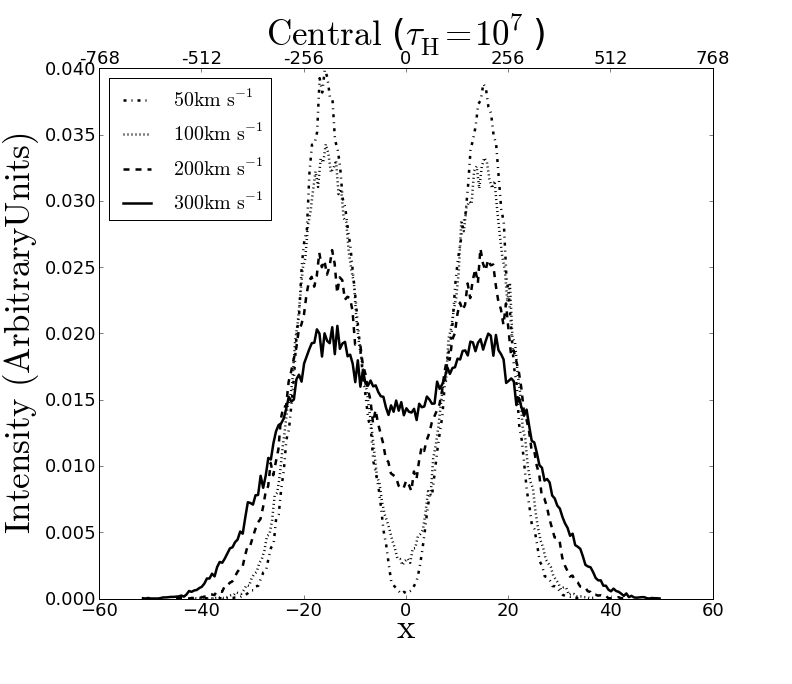
\includegraphics[width=0.45\textwidth]{SpectraDifVelocitiesCentral.png}
  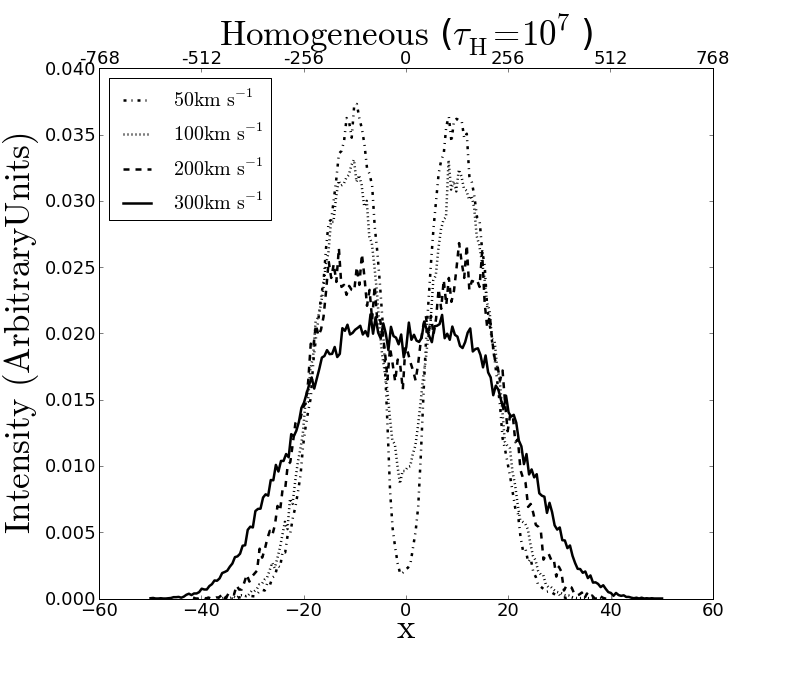
\includegraphics[width=0.45\textwidth]{SpectraDifVelocitiesHOM.png}
\caption{Shape of the \ly line for
    different velocities rotational velocities for spherical
    distributions with $\tau_{H}=10^{7}$. The left (right) panel shows
    the central (homogeneous) photon distribution. All photons were
    taken into  account regardless of their final direction of propagation.
    \label{fig:differentvelocities}}  
\end{figure*}

The central result of this paper is summarized in Figure
\ref{fig:differentvelocities}. It shows the considerable
impact of rotation on the morphology of the emergent \ly line. Both
panels in the Figure focus on the results for $\tau_{H}=10^{7}$,
showing that the influence of rotation is present both when the
photons are either homogeneously or centrally initialized over the gas
volume. 

In the following subsections we characterize the line morphology by
the half-width at half intensity and the peak maxima. In order to
interpret the morphological changes in the line we also report the
median number of scatter for each \ly photon in the
simulation. For the models where dust is included we measure the bulk
escape fraction as a function of rotational velocity. Finally, we make
an estimate of the anisotriopic emission of the models in comparison
with static spheres.


\subsection{Line width and peak maxima}
\label{sec:widthpeak}


\begin{figure}
    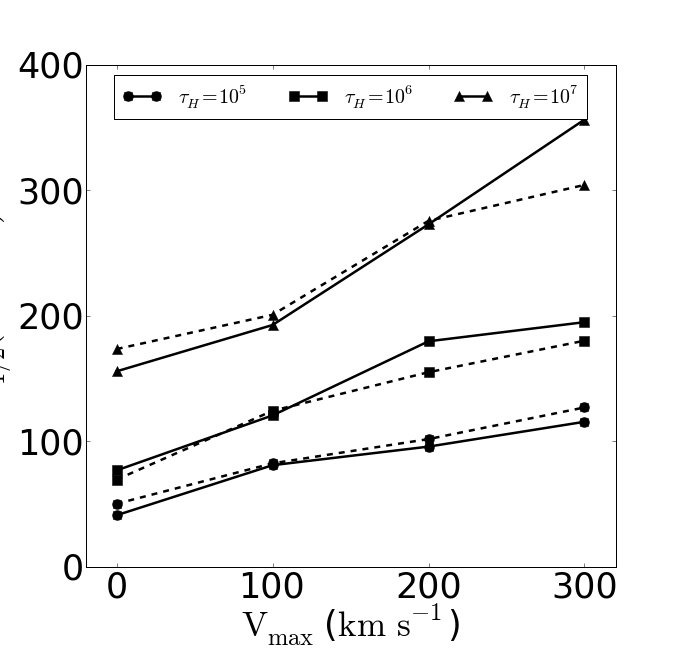
\includegraphics[width=0.45\textwidth]{WidthVvsVmax.png}
    \caption{Half-width for the non-dusty models as a function of
      rotational velocity $V_{\rm max}$. Continuous (dashed) lines
      correspond to homogeneous (central) source
      distributions. \label{fig:widthvsvelocity}} 
\end{figure}


\begin{figure}
    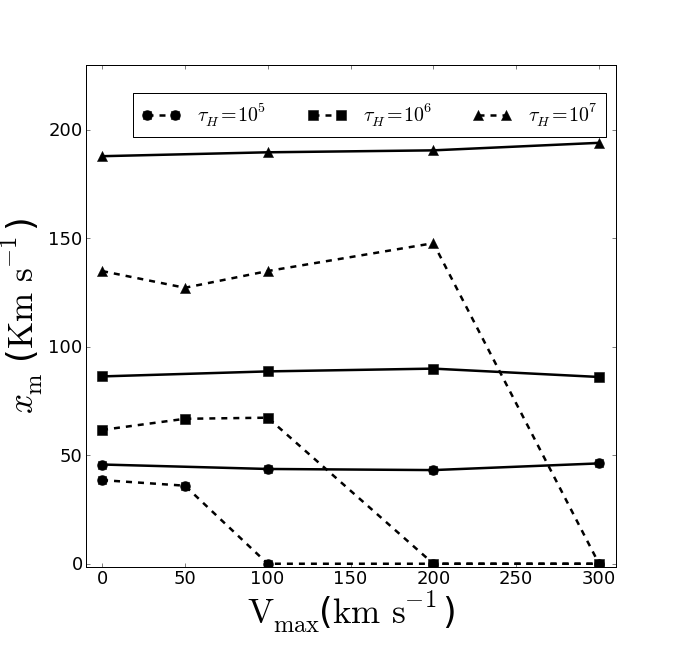
\includegraphics[width=0.45\textwidth]{maximumVvsVmax.png}
\caption{Position of the peak maxima as a function of rotational
  velocity $V_{\rm max}$. Continuous (dashed) lines correspond to
  homogeneous (central) source distributions. A value of $x_{\rm
    max}=0$ indicates that line becomes single
  peaked. \label{fig:maximumsvsvelocity}}  
\end{figure}

The first quantitative conclusion of the effect of rotation in the
\ly line is that double peaks broaden and reduce their intensity
while the line center rises. This produces the impression that, as the
rotational velocity increases, the double peaks are merged into a
single broad emission peak. This is most evident at the highest
rotational velocities for the homogeneously distributed sources
(right panel in Figure \ref{fig:differentvelocities}). 

To quantify the line broadening we use a modified version of the full
width at half maximum (FWHM). We measure it only for half of
the line, $W_{1/2}$. This definition allows us to quantify the line
width and see the transition from double to single peak emission.  In the
case of double peaked emission $W_{1/2}$ corresponds to the width of a
single peak, while in the extreme case of high rotational velocities,
when the double peak is erased, it simply correspond to half FWHM.  

Figure \ref{fig:widthvsvelocity} shows how $W_{1/2}$ increases with
rotational velocity. Continuous (dashed) lines connect the results for
homogeneous (central) source distribution. For the temperature
$T=10^4$K used in our radiative transfer calculations the thermal
velocity is $v_{th}=12.8$\kms. For a model with $\tau_{H}$ it means
that the half-width can increase up to $350$\kms (at $V_{\rm
  max}=300$\kms) compared to a half-width of $150$\kms in the static
case.   

Figure \ref{fig:maximumsvsvelocity} shows the position for the peak
maxima as a function of the rotational velocity $V_{\rm max}$. This
Figure clearly shows that in the case of central distributed
sources there is barely any change with rotational velocity in the
range of explored parameters. However, in the case of
homogeneously emitted sources the maxima position remain close to
constant until beyond some velocity threshold the line becomes single
peaked with $x_{\rm max}=0$ \kms. 

The transition to a single peak line seems to occur for systems
where it becomes easier for the bulk of the photons to escape with the lowest
number of scatterings possible, allowing them not to move very far
from the center of the line. This might explain how the single peak stage
is easily achieved in the homogeneous source distribution. In this
case there is a fraction of the photons that are inside a photosphere
region with $\tau_{H,r}\ll \tau_{H}$ where $\tau_{H,r}$ is the optical
depth from the radius of emission to the sphere's surface. This
conditions allows the photons to escape with much less scatterings
compared to the photons emitted at the very center of the sphere. In
turn, it gives the photons less scatterings to be placed far from the
line center. 

Increasing the rotational velocity $V_{\rm max}$ reduces
the optical depth making the photosphere region effectively larger,
increasing the number of photons escaping close to the lines's
center. In our models we find the following correspondence between the
optical depth $\tau_{\rm H}=\{10^5, 10^6, 10^7\}$ and the transitional
velocities $V_{\rm   trans}=\{50-100\kms, 100-200\kms, 200-300\kms\}$
which can only be constrained to be in the range of velocities in the
models that gave a $x_{\rm max}\neq 0$ and $x_{\rm max}=0$.  


For the central emission the transition to a single peak is never
completed in the range of parameters explored here. The nonappearence
of a single peak phase can be in part explained to the absence of a
photosphere, as is the case in the homogeneous
distribution. Nevertheless, there is a rise in the intensity at the
line center as the rotational velocity increases. This hints that the
encounters with a nonstatic medium are inefficient in changing a
photons' frequency outside the line center.

In the next section we quantify the number of scatterings and explore
to what extent this is related to the emergence of single peak. 

\subsection{Average Number of Scatterings}


\begin{figure}
    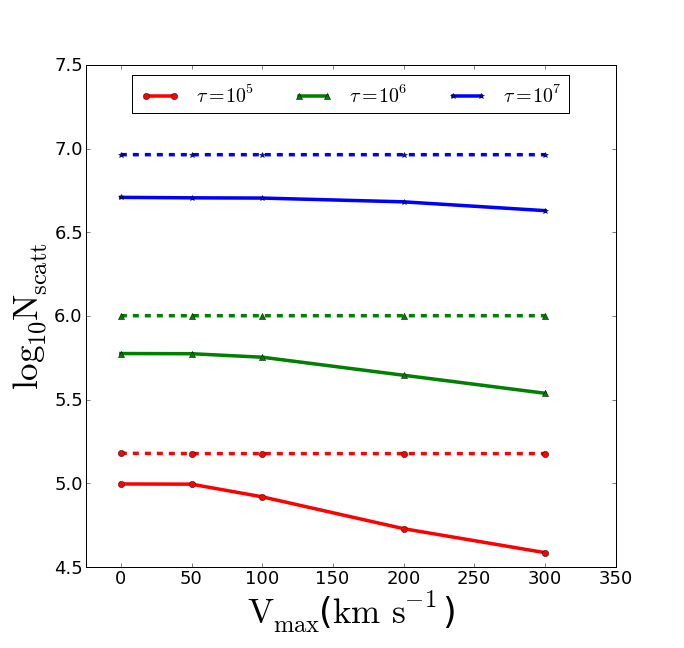
\includegraphics[width=0.45\textwidth]{NscattvsVmax.png}
\caption{Logarithm of the average number of scatterings as function of
  the velocity. Continuous/dashed lines represent an
  homogeneous/central distribution of sources. \label{fig:Nscatt}}    
\end{figure}


\begin{figure*}
     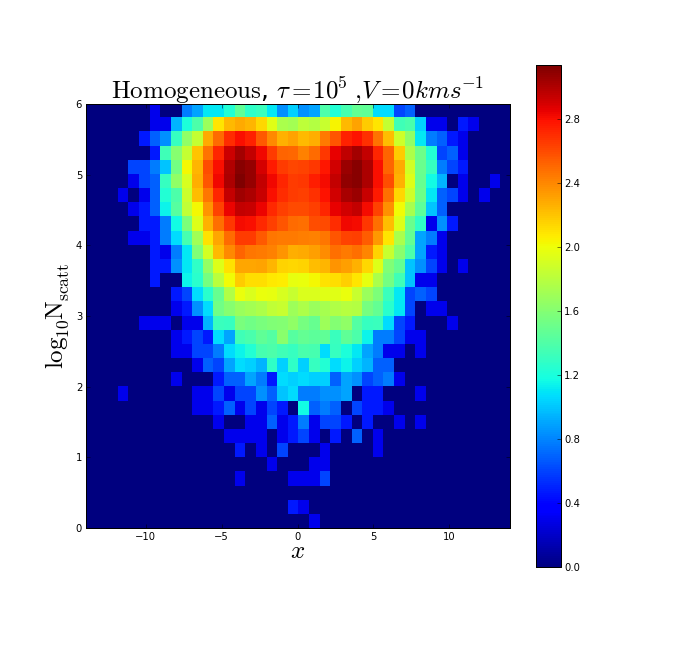
\includegraphics[width=0.45\textwidth]{2dHistogram0t5HOM.png}
     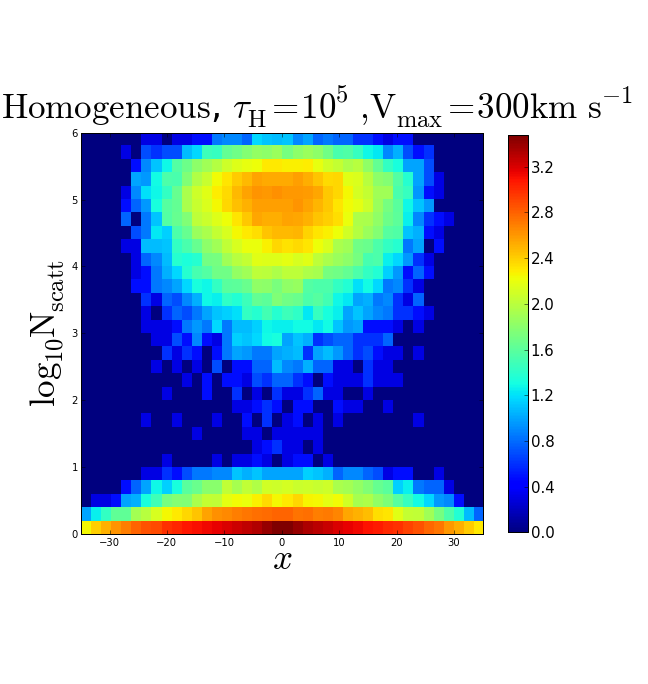
\includegraphics[width=0.45\textwidth]{2dHistogram300t5HOM.png} 
     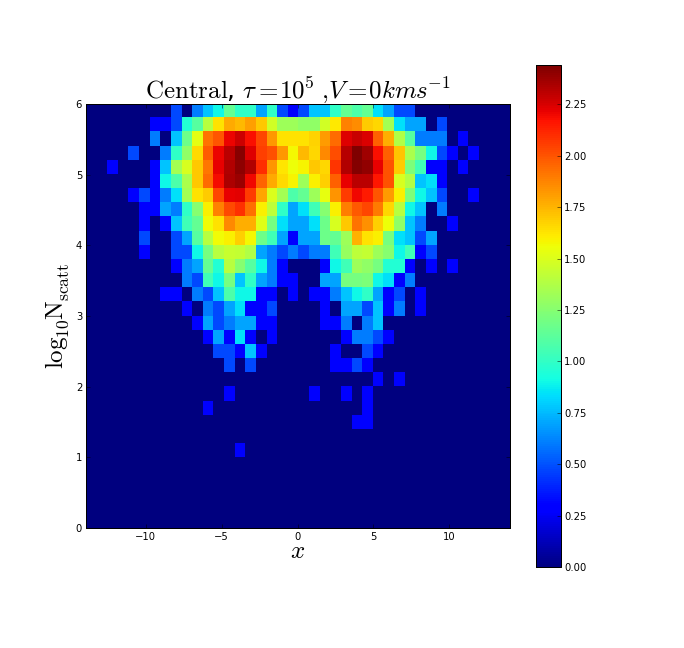
\includegraphics[width=0.45\textwidth]{2dHistogram0t5.png}
     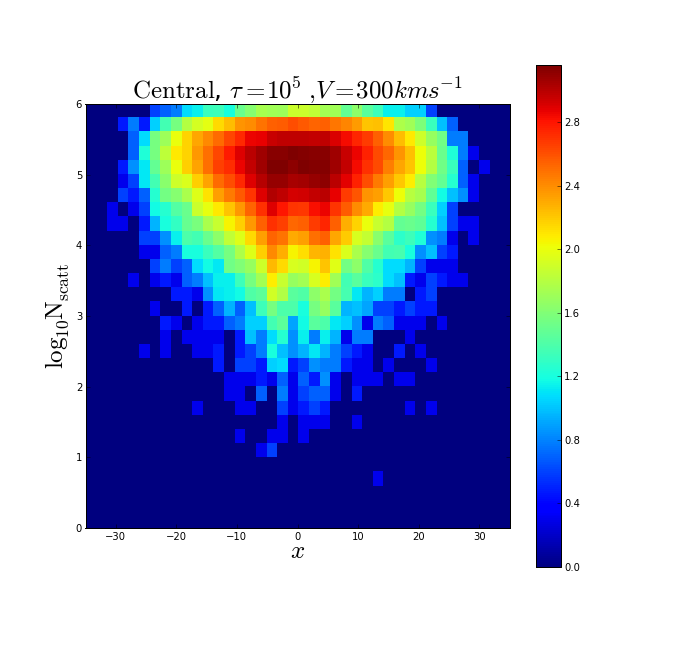
\includegraphics[width=0.45\textwidth]{2dHistogram300t5.png}    

    \caption{2D histogram of $N_{\rm scatt}$ vs $x$. The upper (lower) pannels
      show the homogeneous (central) source distribution. Left
      corresponds to the static case and the right
      $V_{max}=300km/s$. The colour scale is logarithmic on the
      number of photons with given values of $N_{\rm scatt}$ and
      $x$. \label{fig:Nscatt2D}}   
\end{figure*}


The number of times that a \ly photon is absorbed and re-emitted is
connected to the final frequency that it can have after escaping the
galaxy. In the case of static gas geometries, a large value of the
optical depth is immediately followed by a high number of
scatterings. In turn a large optical depth increases the probability
that a \ly photon to be found far from the center of the line. In this
case, the peak maxima shift away form the line center as the amount of
neutral hydrogen increases.


In Figure \ref{fig:Nscatt} we show the average number of scatterings
$\langle N_{\rm scatt}\rangle$ as a function of the rotational velocity
$V_{\rm max}$. For the central distributions we find that there is not
a significant change for increasing rotational
velocities, $\langle N_{\rm scatt}\rangle$ changes less than $0.5\%$
for different velocities. In this case we also find that the average
number of scatterings is proportional to the optical depth, as
expected in analogy from the analytic result for the homogeneous
infinite-slab $\langle N_{\rm  scatt}\rangle=1.612\tau_{\rm   H}$
\citep{Adams72,Harrington73}. In our experiments we find  that for the
static spheres with centraly distributed sources $\langle N_{\rm
  scatt}\rangle= (1.50, 1.00, 0.92)\tau_{\rm   H}$. for optical depths
$\tau_{\rm H} = (10^{5}, 10^{6}, 10^{7})$


Figure \ref{fig:Nscatt} shows that for the homogeneous distribution
there is a clear decrease of $\langle N_{\rm  scatt}\rangle$ as the
$V_{\rm max}$ increases. This effect more pronounced for the lower
values of the optical depth. For $\tau_{\rm H}=10^5$ the average
number of scatterings decreases by $61\%$ at $V_{\rm max}=300\kms$ in
comparison to the static case. 

The analytic expectation for the slab with homogeneously emitted
sources is $\langle N_{\rm  scatt}\rangle=1.16\tau_{\rm   H}$
\citep{Harrington73}, a factor of $0.72$ lower than the case of the
centrally emitted photons. In our case we find that for the static
, while for homogeneously distributed source $\langle N_{\rm
  scatt}\rangle= (0.99, 0.59, 0.51)\tau_{\rm   H}$, this represents 
  a factor of $(0.66, 0.59, 0.51)$ lower than the centrally emitted photons.

In order to gain a deeper understanding of these results we prepare 2D
histograms for the number of scatterings as a function of the outgoing
dimensionless frequency $x$. In Figure \ref{fig:Nscatt2D} we show
the results of such histogram in the case $\tau_{\rm H}=10^5$ for the
static case and $V_{\rm max}=300$\kms. The upper (lower) panels show the
results for the homogeneous (central) source distribution. The color
scale is logarithmic in the number of photons at a certain value
$x-N_{\rm scatt}$. This Figure clearly support our hypothesis about
the photosphere in the homogeneous distribution, in this case most of
the photons that left with $x\sim 0$ have escaped with less than $10$
scatterings, explaining the origin of a single central
peak. However, for a central distribution the situation is
different. In this case the number of scatterings remains high, on the
order of the optical depth, but the two peaks do get closer to each
other. In this case the physical picture is that each scattering, due
to the bulk velocity of the gas, is inefficient in driving the photon
outside the line center.


\subsection{Dusty Clouds: Escape Fraction}
\label{sec:escapefraction}


\begin{figure}
  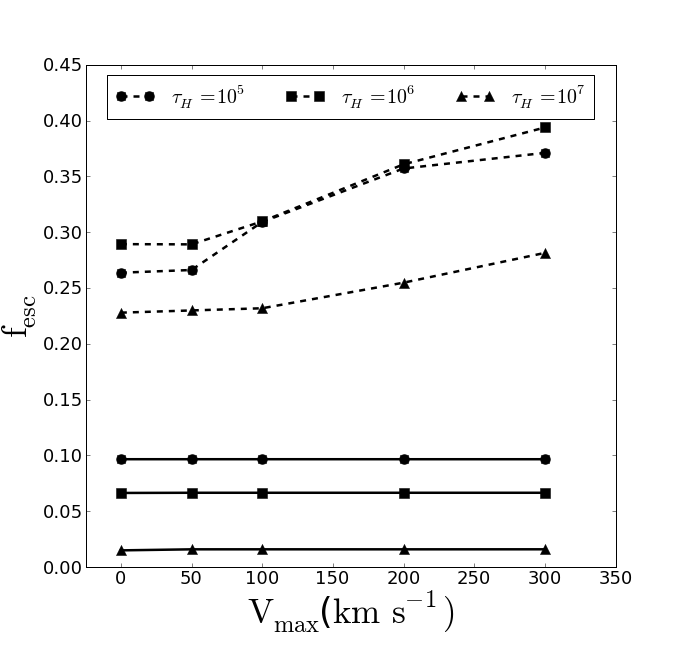
\includegraphics[width=0.45\textwidth]{escapefraction.png}
   \caption{Escape fraction as a function of rotational velocity. The
     continuous (dashed) lines correspond to homogeneous (central)
     models.
     \label{fig:efvsv}}
\end{figure}


\begin{figure}
  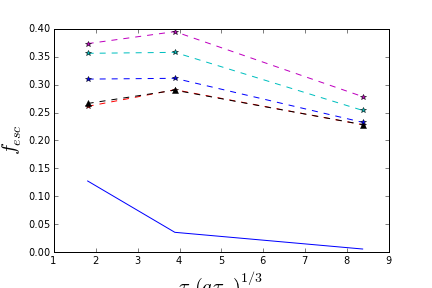
\includegraphics[width=0.45\textwidth]{Neufeld.png}
 \caption{Escape fraction as a function of the
   product $(a\tau_{\rm H})^{1/3}\tau_{a}$. The analytic solution for
   the infinite is slab shown as a continuous line. Different dashed
   lines correspond to different rotational velocities.
   \label{fig:efvsNeufeld}}   
\end{figure}

We also study a dusty cloud configuration to measure the effect of
rotation on the escape fraction. We expect that the modified number of
scatterings to be reflected in this amount of photons absorbed by
dust. Following this line of thought,  we do not expect any change in
for a dusty cloud with central source of radiation given that the
number of scatterings remains close to constant. On the other hand, in
the case of an homogeneous radiation source the number of scatterings
drops as $V_{\rm max}$ increases, which might be reflected as an
increasing escape fraction.

%If there is a change in the number of scatterings with rotational
%velocity, there must be a change in the probability of being absorbed
%if dust is present. We study how rotation impacts the escape fraction
%of \ly photons. 

%Taking into account the results in the previous section, we do not expect any
%change in the case of central distributions given that the average
%number of scatterings remain constant. On the other hand, in the
%homogeneous distribution there is a considerable drop in the number of
%scatterings as $V_{\rm max}$ increases, this preconditions the escape
%fraction to increase as well.

Figure \ref{fig:efvsv} shows the dependence of the escape fraction as
a function of the maximum rotational velocity, confirming that our
intuitions in this respect is correct. For the central source
distribution the escape fraction barely shows any change, while for
the homogeneous case there is a clear rise in the escape fraction for
high rotational velocities.  Rotation has a higher relative impact in
the models with low optical depth $\tau_{\rm H}=10^5$,$10^{6}$, where
it can raise from $(0.26, 0.28)$ respectively in the static case up to $(0.37, 0.39)$ at $V_{\rm
  rot}=300$\kms. 


%This Figure illustrates how our
%reasoning in the previous paragraph is correct. 
%The escape fraction
%barely changes for the central source distribution, while it rises
%as the velocity $V_{\rm max}$ increases for the homogeneous case. 


In Figure \ref{fig:efvsNeufeld} we put these results in the context of
the analytical solution for the infinite slab \citep{Neufeld90}. In
Neufeld's setup the analytic solution depends solely on the product
$(a\tau_{\rm   H})^{1/3}\tau_{a}$, an approximation that is valid only
in the limits $a\tau_{\rm   H}\gg 1$. The dashed lines in Figure
\ref{fig:efvsNeufeld} correspond to the cases of different
velocities. We observe that the escape fraction is higher
by factors of $2-10$  than the expected values for the slab
configuration. We also see that for the lower value $\tau_{\rm
  H}=10^{5}$ the escape fraction does not increase with respect to the
solution for $\tau_{\rm H}=10^{6}$ as expected, however we not that we
are in a regime where the condition for the analytic expectations 
($a\tau_{h}\gg 1$) does not hold.



\subsection{Anisotropic emission}

We study the deviations of the received flux on the surface of the
sphere. We follow \cite{Zheng2013} to estimate the flux seen by an
observer located at an angle $\Theta$ (distant observer angle)
normalized to the isotropic flux:

\begin{equation}
F(\mu) = \frac{2\Delta N}{N\Delta \mu}, 
\end{equation}
%
where $\mu=\cos\Theta$, $N$ is the total number of outgoing photons,
$\Delta N$ is the number of photons in a angular bin $\Delta
\Theta$. This definition satisfies the condition
$\int_{-1}^{1}F(\mu)d\mu/2=1$. 

In Figure \ref{fig:flux} we show the angular dependency of the flux for the
central (left) and homogeneous (right) source distributions. This
shows that observers at different directions would infer luminosities
different from the isotropical value only at levels $< 3\%$. 

\begin{figure*}
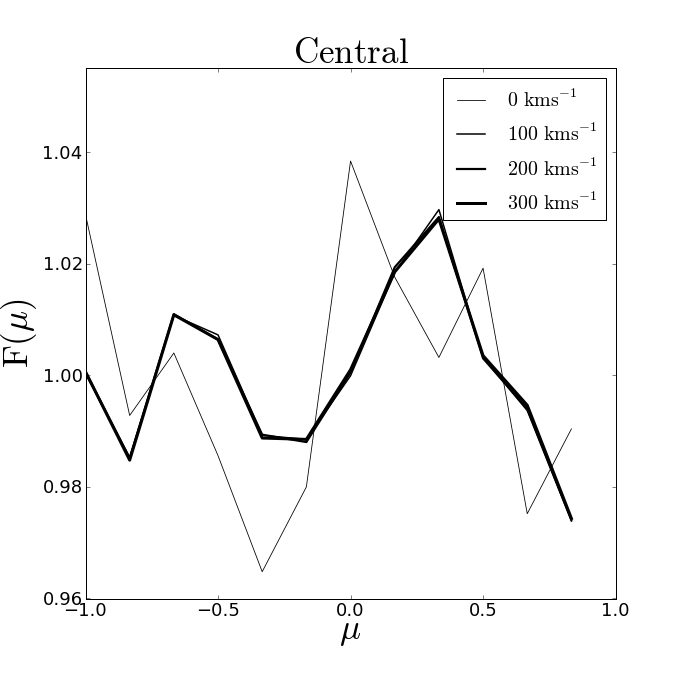
\includegraphics[scale=0.3]{mu_central.png}
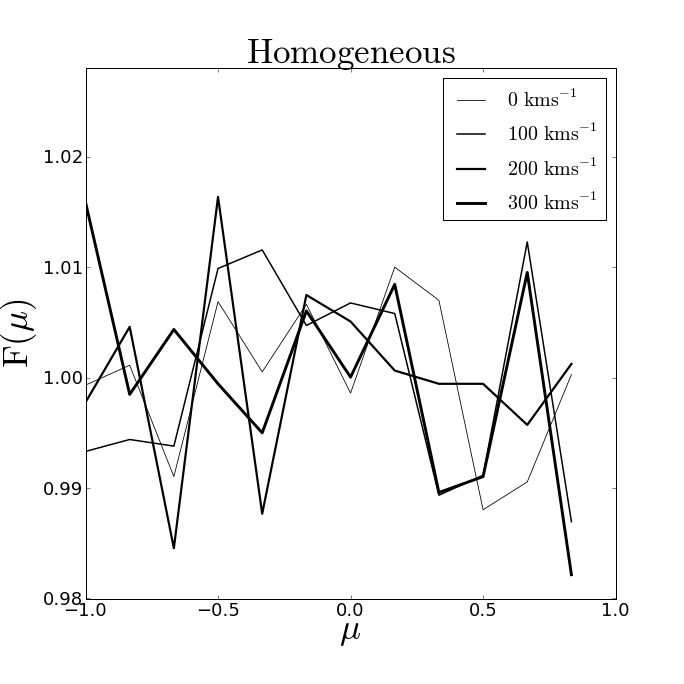
\includegraphics[scale=0.3]{mu_homogeneous.png}
\caption{Flux angular dependency for the central (left) and homogeneous
(right) source distributions, different line widths illustrate different
rotational velocities.
   \label{fig:flux}} 
\end{figure*}

\subsection{Off-Centered emission}

As we know there is unlikely to find galaxies with radiation sources 
distributed homogeneously. Most of them are in a clumpy distribution 
(Laursen et al 2013*) which affected the resulting spectra. In order 
to study an inhomogeneous distribution we set up a model in which we 
select certain photons that are placed in a specific place but that 
are not symmetrically distributed Fig. \ref{fig:OCspheres} shows the distributions we 
set up, basically we take photons located in a sphere of $0.5 R$ and 
we choose two speheres in each side of the $\hat{\textbf{x}}$ axis
two at $0.25 R$ and the other two at $0.5 R$

\begin{figure}
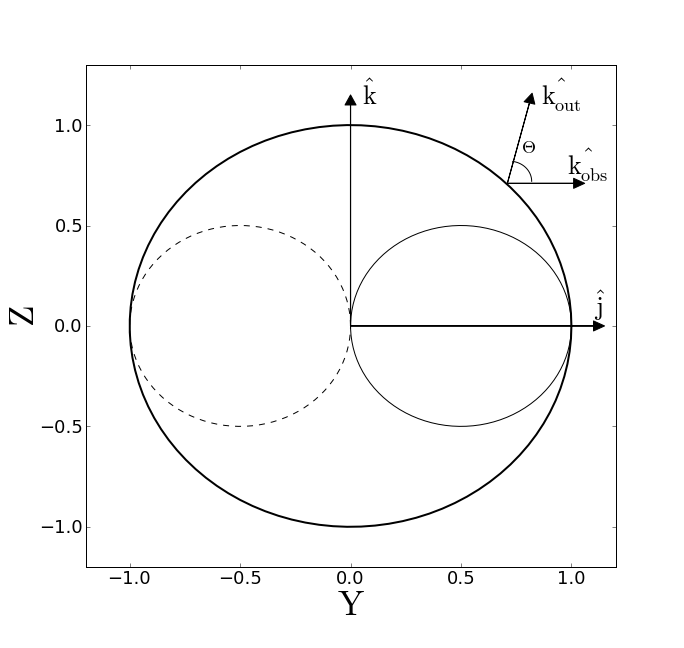
\includegraphics[scale=0.3]{OF_spheres.png}
\caption{The two solid circles show up the photons we select in order to make the anisotropic emission
		rotation is defined to be $\mathrm{z}$-axis. we also select photons in the negative side of 				        $\mathrm{x}$ (dashed circles) in order to see the complete effect of rotation. 
   \label{fig:OCspheres}} 
\end{figure}

As a primer approach we study the angular dependency in the same manner as
we do in section(). In Fig. \ref{fig:OCflux} the angular for two different
off-center distribution the bold line shows an off center sphere located
at $0.5 R$ of the homogeneous sphere, while the narrow line shows sphere 
located at $0.25 R$. This is done for the model with $\tau=10^{5}$ and 
$V=50 km s^{-1}$, we find that the maximum change in flux would be up to. 


\begin{figure}
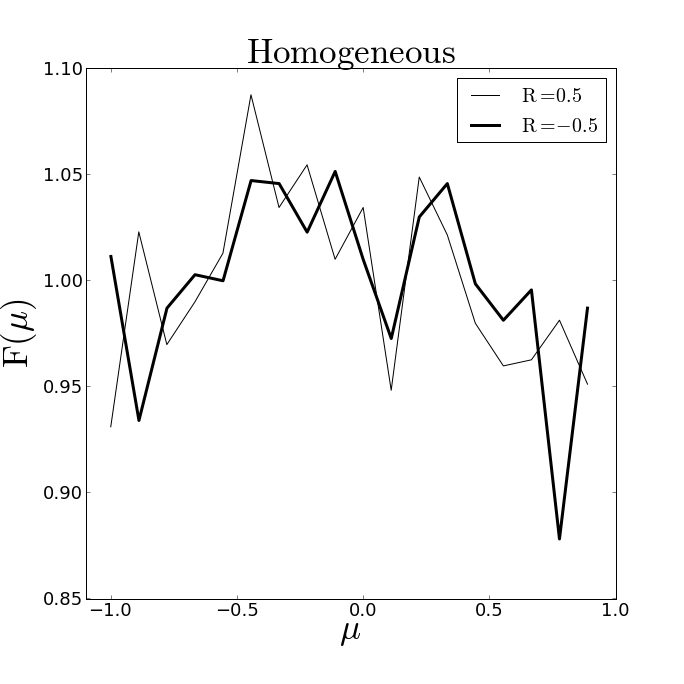
\includegraphics[scale=0.3]{mu_OC.png}
\caption{Flux angular dependency for Off-center distribution, different line widths illustrate different
off-center positions.
   \label{fig:OCflux}} 
\end{figure}

The outgoing spectra for two different spheres located at $-0.25R$ and $0.25R$ respectively
is shown in Fig. \ref{fig:OCspectra}, we have shown this positions because
they are the most sensitive to rotational velocities.
\begin{figure}
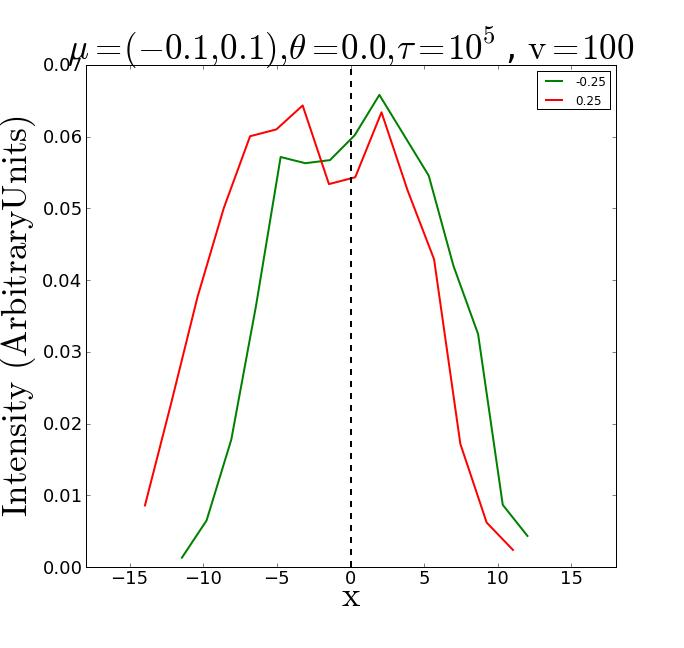
\includegraphics[scale=0.3]{OC_5t_vel100.jpg}
\caption{Spectra for two off-center spheres
   \label{fig:OCspectra}} 
\end{figure}

There are two new morphological featueres that off-center emission in 
rotating galaxies produces. First in some of our models with especific 
values of velocity and opitcal depth an asymmetry in the peak heights 
is presented, those off-center spheres \textit{(put image reference)} 
located at the positive side of $\hat{\textbf{x}}$ in Fig.\ref{fig:OCspheres}
present a higher peak in the redshifted part, while those spheres located
at the negative side of $\hat{\textbf{x}}$ present a higher blue shifted peak,
we found that the higher asymmetry is for model with $\tau=10^7, V=200 kms^{-1}$ where one peak is $20\%$ higher than the other.
This can be apreciated for both set of spheres at $0.25 R$ and $0.5 R$,
 but the effect shows a stronger asymmetry for spheres located at $0.25 R$
 this due to the fact that photons escaping from this spheres goes through 
 a larger hidrogen medium than photons located in the spheres at $0.5 R$.
%poner valores de velocidad y optical depth porcentaje de asimetria 

Also for all the off-center models we found that the $Ly\alpha$ line 
width ...
 
 
Also for photons located in the spheres at $0.5 R$, we found that for 
some models ($\tau = 10^6, V=100 km s^{-1}$ and $\tau = 10^7, V=200 km s^{-1}$)
the line presents three peaks (blue-shifted, centered, red-shifted). In order to gain a better interpretation of this three peaks trend we run this models with $N_{\gamma} = 10^6$.
 


%\begin{figure}
%  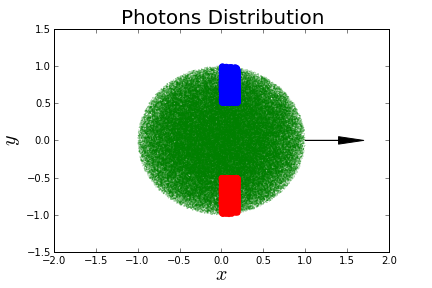
\includegraphics[width=0.40\textwidth]{Distribution.png}
%  \caption{Inhomogeneous distributions of 
% photons, Blue area represents the photons in distribution 1 while red
% area are the selected photons for distribution 2. The arrow points to
% the observer position\label{figure:distributions}}  
%\end{figure}

%In Fig.~\ref{figure:inhomogeneous} we show the resulting spectra of 
%distribution 1 and 2, the first effect we see is the asymmetry of the
%double peak, in the homogeneous and central distribution we see double
%peaks with the same height, while in this case one peak is higher than 
%the other. For $\tau=10^{5}$ we found that in distribution 1 the blueshifted
%peak is higher than the reds~\ref{figure:distributionshifted, and for distribution 2 the redshifted
%peak is the highest.

%An other important fact here is the asymmetry of the spectra with respect 
%to the line center, in particular photons selected in distribution 1 
%present a blueshift in their spectra while photons selected in distribution 
%2 present a redshift. This effect becomes stronger as velocity increase 
%~\ref{figure:inhomogeneous}
 
%\begin{figure*}
%  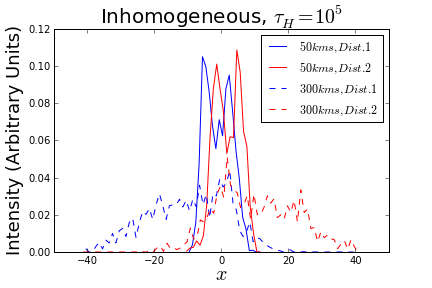
\includegraphics[width=0.45\textwidth]{InomogeneousModelt5.png}
%  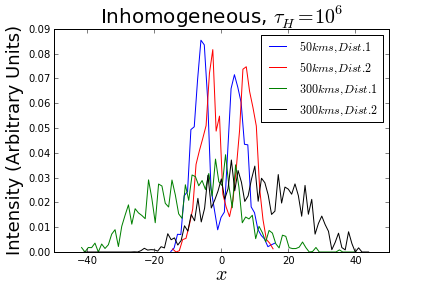
\includegraphics[width=0.45\textwidth]{InomogeneousModelt6.png}
% \caption{Inhomogeneous model for velocities $50km/s$ and $300km/s$ ,
%   (left) with $\tau=10^5$, (right) with
%   $\tau=10^6$\label{figure:inhomogeneous}}  
%\end{figure*}
 

%\subsection{Integrated flux in a narrowband filter}

%Until now we have shown the main effects of gas and dust rotation in
%the Ly$\alpha$ line morphology such as the escape fraction, the FWHM,
%the maxima position, also we see that shape of the outgoing spectra
%depends on the position of the observer. It is important to see if
%rotational effects are detectable in observational methods involving
%the Ly$\alpha$ line.  

%One of the most used methods to detect high redshift galaxies using
%the Ly$\alpha$ line is using a narrowband selection, we make this
%analysis based on the results obtained by Steidel (2011) in this work
%(EXPLAIN a lit of bit more about their work) they used tree narrowband
%filters for tree different redshifts resumed in
%Table~\ref{table:NBfilters}, We want to know how much the integrated
%flux change due to rotational effects in this NB filters, for the
%models we simulated with CLARA. 

%\begin{table*}
%\begin{center}
%\begin{tabular}{cccc}\hline
%Model & SSA22a 4980/80   & HS1549 4667/80 & HS1700 4018/90\\
%\hline
%\end{tabular}
%\caption{
%Fluxes for tree different narrow band filters.
%} 
%\label{table:NBfilters}
%\end{center}
%\end{table*}

%In table \ref{table:NBfilters} we present the results of the flux in
%every  narrowband filter for the homogeneous model at different
%velocities and hydrogen  optical depth $\tau_{0}$. As is well known an
%increase in the optical depth makes  the line peaks separation
%bigger. In fact for some cases the line width is larger  than the NB
%filer width fig.(put ref fig) for those cases we modify the redshift
%in the available range in order to make the peak maxima match the NB
%filter center.  For all cases we found that as velocity increase the
%flux is less.  

%In the case of the dusty model we found the same trend of the flux
%with the velocity  but in this cases the effect is no that strong.  We
%also found some dependency with the viewing angle. 

%\begin{figure}
%  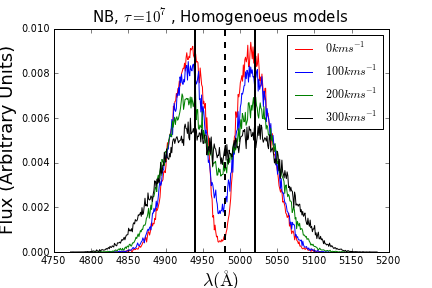
\includegraphics[width=0.45\textwidth]{NB7tDifVHOM.png}
% \label{figure:efvsNeufeld}\caption{NB filter located at the center of
%   the maxima, with different redshift}  
%\end{figure}

\section{Discussion}
\label{sec:discussion}

... Comparison with Verhamme et al. results on the rotation (Viewing angle)


... Compare with Kulas et al (Figure 3), Rotation on the lyman alpha
line convert double peak profiles into a single one. comments about
rotation with inflows and outflows.   

... The results derived in this paper have consequences on the
interpretation of galaxy observations in the Lyman alpha line.

..compare steidel et al (2011) 

% BUSCAR asimetrias en observaciones, KUlas, YAMADA  off-center emission

% taking into account equivalent widths results with narrow band
% filters we can make a criterium in order to select wich galaxie
% could be seen in actual observations.  



\section{Conclusions}
\label{sec:conclusions}
In this paper we have estimated the effects of gas bulk rotation on
the emission  of the Lyman $\alpha$ line. We based the study on the
study of a simplified configuration of an homogeneous sphere rotating
as a solid body. We explored  a range of models by varying the
rotation speed, hydrogen optical depth, dust optical depth and initial
distribution of Ly$\alpha$ photons with respect to the gas
density. This was implemented in CLARA, a Monte-Carlo
radiative transfer code already used to study the Lyman $\alpha$
line. 

As first we see how the width of the line changes using a modified FWHM
explained in section \ref{sec:widthpeak}, and we found that as gas bulk 
rotation increase also the width increase in a factor of $2-3$ in comparison 
with the static case. 'We also take into account the influence of the observer 
viewing angle, we found that observers with a line of sight perpendicular  
to the axis of rotation measure a $15\%$ larger line width than those 
aligned with the rotation axis.'

As many observational spectra Ly$\alpha$ emission line (Kulas et al, Yamada et al)
is double  peaked, these peaks provide important information
concerning gas kinematics and geometry,  which can be partially
explained with inflows/outflows of gas content.  We study the effect
of rotation in the position of this peaks, and we find  that the
position of the maxima does change with rotation for the homogeneous
models when the double peak merged into a single peak as velocity
increase. This effect is not seen for the central distribution when
the double peak  remains constant as the velocity increase. We also
find that there is no dependency in the observer viewing angle with
the maxima position. 

Concerning the escape fraction under rotational effects on the
Ly$\alpha$ emission line, we found that the escape fraction increase
in about $20\%-30\%$for the homogeneous sphere model. While rotational
effects are negligible for the central models and the escape fraction
remains constant. Also the observer viewing angle have no effect in
the escape fraction neither for the homogeneous and central
models. Complementing this analysis we study the average number of
scatterings $<N_{scatt}>$ that photons perform before escaping of the
cloud taking into account rotational effects. The main result here is
for the homogeneous models for which as velocity increase photons
escape with about $\sim 39\%$  less scatterings than in the static
case. 

%As an application of these results we compute the integrated flux
%taking into account the narrow band filters used by (Steidel et al
%2011), for our models we found an important decrease up to $~40\%$ for
%the homogeneous models, and up to $22\%$ for the dusty homogeneous
%models in the flux as velocity increase.  Also we calculate at what
%redshift should the filter be in order to get the maximum  flux, and
%for the tree filters we get values that rely in the filter redshift
%range. This effects would have a relevant implication at the time to
%find high redshift galaxies.

This paper illustrates for the first time the main effects of rotation
in the morphology of the Ly$\alpha$ emission line, we estimate the
range of this effects for simplified models.


\section*{Acknowledgements}


\bibliography{references} 

\section*{Appendix A: Tables}


\end{document}



%ideas:
Keep in mind making a follow up paper on the results of Yamada et atl
http://adsabs.harvard.edu/abs/2012ApJ...751...29Y on the line
morphology at z=3.1. How many of t hese laes can be considered to have
rotation features? In principle, all of then should have them. How to
make the case convincing in the statistical sense? 

